
\section{Auswertung}
\subsection{Bestimmung des Winkels $\su{\varphi}$}
Zur Bestimmung des brechenden Winkels $\su{\varphi}$ werden die Winkel $\su{\varphi_{links}}$ und $\su{\varphi_{rechts}}$
der beiden reflektierten Strahlen aufgenommen. In Tabelle \ref{tab:phi} sind die Messwerte $\su{\varphi_{links}}$ und
$\su{\varphi_{rechts}}$ aufgetragen. Der daraus resultierende Winkel $\su{\varphi}$ wird mit Formel \ref{eqn:phi} berechnet
\begin{table}
\centering
\caption{Messwerte für $\su{\varphi}$}
\label{tab:phi}
\begin{tabular}{S S S S}
\toprule
{Messung} & {$\su{\varphi_{links}}\,/\,^\circ$} & {$\su{\varphi_{rechts}}\,/\,^\circ$} & {$\su{\varphi}\,/\,^\circ$} \\
\midrule
 1 & 96,6 & 216,7 & 60,05 \\
 2 & 101,4 & 221,6 & 60,10 \\
 3 & 99,0 & 219,0 & 60,00 \\
 4 & 107,1 & 227,3 & 60,10 \\
 5 & 106,7 & 227,0 & 60,15 \\
 6 & 100,8 & 221,0 & 60,10 \\
 7 & 101,0 & 221,4 & 60,20 \\
\bottomrule
\end{tabular}
\end{table}
\newline
Für den Winkel $\su{\varphi}$ ergibt sich aus
\begin{equation*}
  \bar{\varphi} = \frac{1}{n} \sum{\varphi_n}
  \label{eqn:Mittelwert}
\end{equation*}
und
\begin{equation*}
\upsigma = \frac{1}{\sqrt{n}} \sqrt{\frac{\sum{(\varphi_n - \bar{\varphi})^2}}{n-1} }.
\label{eqn:Standardabweichung}
\end{equation*}
der Wert $\su{\varphi} = (60,10\pm0,03)^\circ$.

\subsection{Bestimmtung des Winkels $\upeta$ und der Brechungsindices n}
Die gemessen Winkel $\su{\omega_{rechts}}$ und $\su{\omega_{rechts}}$ sind in Abhängigkeit
der Wellenlänge in Tabelle \ref{tab:beta} dargestellt.
\begin{table}
\centering
\caption{Messwerte zur Bestimmung von $\upeta$ und n}
\label{tab:beta}
\begin{tabular}{S S S S S}
\toprule
{Wellenlänge} & {$\su{\omega_{rechts}}\,/\,^\circ$} & {$\su{\omega_{links}}\,/\,^\circ$} & {$\upeta$} & {n}\\
\midrule
 643,84 & 333,3 & 91,0 & 62,3 & 1,750\pm0,046 \\
 576,96 & 333,5 & 90,7 & 62,8 & 1,754\pm0,046 \\
 546,07 & 334,3 & 90,1 & 64,2 & 1,766\pm0,046 \\
 508,58 & 335,0 & 89,6 & 65,4 & 1,775\pm0,046 \\
 479,99 & 335,3 & 88,8 & 66,5 & 1,784\pm0,047 \\
 467,81 & 335,5 & 88,3 & 67,2 & 1,789\pm0,047 \\
 435,83 & 336,3 & 88,1 & 68,3 & 1,798\pm0,047 \\
 404,66 & 337,3 & 87,2 & 70,1 & 1,811\pm0,047 \\
\bottomrule
\end{tabular}
\end{table}
\newline
Mit den Messwerten aus Tabelle \ref{tab:phi} und \ref{tab:beta} können die Brechungsindices für die
einzelnen Wellenlänge durch
\begin{equation*}
  n= \frac{\su{sin}\,{\frac{n+\varphi}{2}}}{\su{sin}\,{\frac{\varphi}{2}}}
\end{equation*}
bestimmt werden. Die Fehler der Brechungsindices ergeben sich mit der Gauß'schen Fehlerfortpflanzung
\begin{equation*}
  \Delta{n} = \sqrt{\Big(\frac{dn}{d\varphi} \Delta\varphi\Big)^2} = \bigg\vert\bigg(\frac{0,5\,\su{cos}\,(\frac{n+\varphi}{2})}{\su{sin}\,(\frac{\varphi}{2})} - \frac{0,5\,\su{cos}\,(\frac{\varphi}{2})\su{sin}\,(\frac{n+\varphi}{2})}{\su{sin^2}\,(\frac{\varphi}{2})}\bigg)\Delta\su{\varphi}\bigg\vert.
\end{equation*}

\subsection{Bestimmung der Dispersionsgleichung}
Um zu entscheiden welche der beiden Dispersionsgleichungen besser zu dem Dispersionsverhalten
der aufgenommenen Messwerte passt, werden die Messwerte und die beiden Theoriekurven in Abbildung
\ref{fig:dispersion} aufgetragen und miteinander verglichen. Dafür werden die Wellenlängen in Abhänigkeit
des Quadrats des Brechungsindex dargestellt.
\begin{figure}
  \centering
  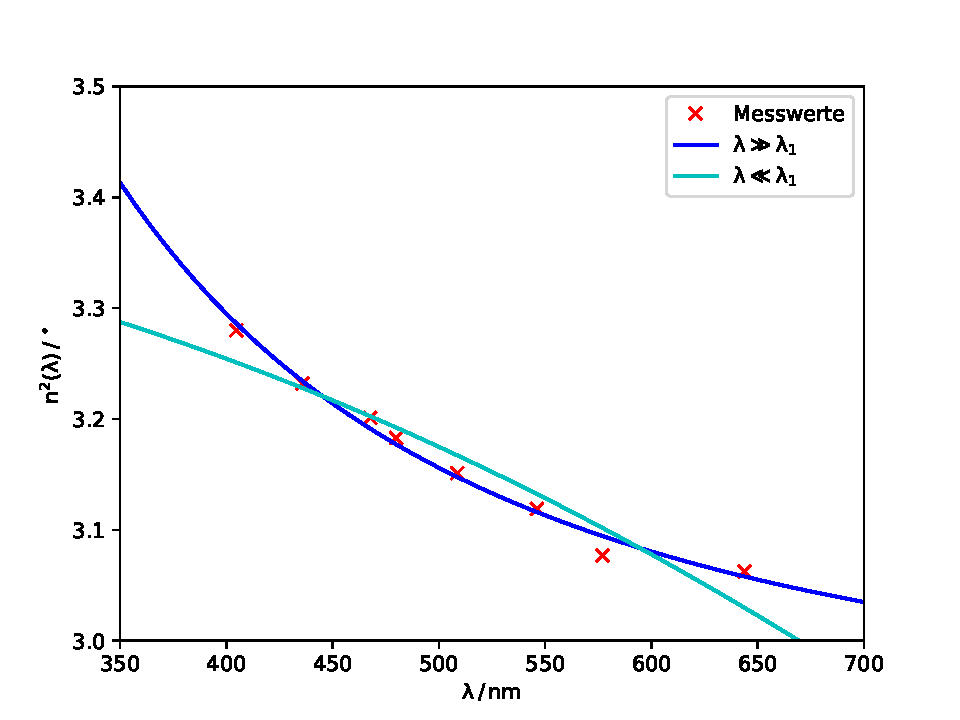
\includegraphics[scale=0.7]{dispersion.pdf}
  \caption{Vergleich der theoretischen Dispersionskurven mit den Messwerten}
  \label{fig:dispersion}
\end{figure}
\newline
Die daraus folgenden Paramater sind aus Tabelle \ref{tab:disp} zu entnehmen.
\begin{table}
\centering
\caption{$\su{Dispersionsgleichung}$}
\label{tab:disp}
\begin{tabular}{S | S S}
\toprule
{Dispersionskurve} & & {Steigung} \\
\midrule
  1 & $\su{A_0}$ & $\num{2.909(13)}$ \\
      & $\su{A_2}$ & $\num{6.18(29)E4}$ \\
  2 & $\su{A_0'}$ & $\num{3.396(29)}$ \\
      & $\su{A_2'}$ & $\num{8.8(1)E-7}$ \\
\end{tabular}
\end{table}
\newline
Damit lassen sich die Abweichungsquadrate durch
\begin{equation*}
  s_n^2 = \frac{1}{z-2}\sum\limits_{i=1}^z\bigg[n^2(\lambda_i)-\su{A_0}-\frac{\su{A_2}}{\lambda_i}\bigg]^2
\end{equation*}
für den Fall $\su{\lambda} \gg \su{\lambda_i}$ berechnen. Die Berechnung für den zweiten Fall $\su{\lambda} \ll \su{\lambda_i}$ erfolgt durch
\begin{equation*}
  s_{n'}^2 = \frac{1}{z-2}\sum\limits_{i=1}^z\Big[n^2(\lambda_i)-\su{A_0'}+ A_2'\lambda_i\Big]^2.
\end{equation*}
Hierbei steht z für die Anzahl der Messwertpaare, die in diesem Teil des Versuchs sieben beträgt.
Für die Abweichungsquadrate folgt dann
\begin{align*}
  s_{n}^2 &= 1,044 \cdot 10^{-4} \\
  s_{n'}^2&= 6,258 \cdot 10^{-4}.
\end{align*}
Dadurch, dass das Abweichungsquadrat für $\su{\lambda} \gg \su{\lambda_i}$ kleiner ist und auch in Abbildung \ref{fig:dispersion}
die Theoriekurve zu den Messwerten passt, kann der Brechungsindex durch die Parameter
\begin{equation*}
  n(\lambda)= \sqrt{\su{A_0}+\frac{\su{A_2}}{\lambda^2}} = \sqrt{2,909+\frac{ 6,18 \cdot 10^{4}}{\lambda^2}}
  \label{eq:n}
\end{equation*}
ausgedrückt werden.
\newline
In Abbildung \ref{fig:dispersionskurve} ist die resultierende Dispersionskurve zusammen mit den Messwerten
dargestellt.
\begin{figure}
  \centering
  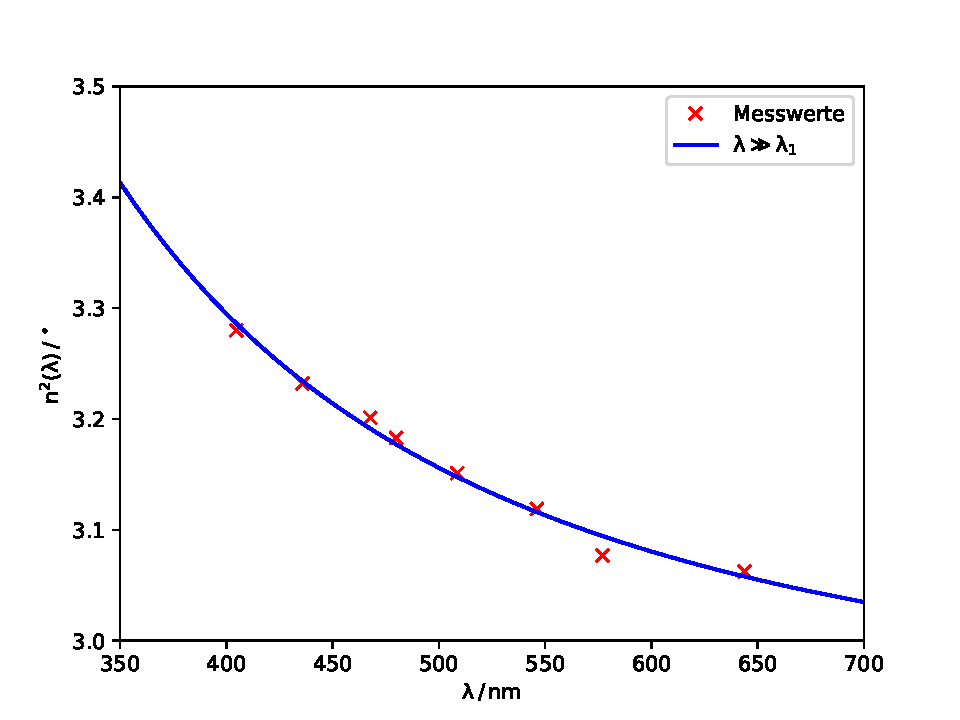
\includegraphics[scale=0.5]{dispersionskurve.pdf}
  \caption{Dispersionskurve}
  \label{fig:dispersionskurve}
\end{figure}
\newpage
\subsection{Bestimmung der Abbeschen Zahl}
Die Brechungsindices für die Fraunhoferschen Linsen werden zuerst mit Formel \ref{eq:n} bestimmt. Die Fehler
der Brechungsindices ergeben sich durch
\begin{equation*}
     \Delta{n} = \sqrt{\bigg(0,5\big(\su{A_0}+\frac{\su{A_2}}{\lambda^2}\big)^{-\frac{1}{2}}\Delta{\su{A_0}}\bigg)^2 + \bigg(0,5\bigg(\su{A_0}+\frac{\su{A_2}}{\lambda^2}\bigg)^{-\frac{1}{2}} \Big(\frac{1}{\lambda^2}-\frac{2\su{A_2}}{\lambda^3}\Big)\bigg)\Delta{\su{A_2}}\bigg)^2}
\end{equation*}
Die sich ergebenden Werte sind in Tabelle \ref{tab:abbe} dargestellt.
%\begin{equation}
%   \Delta{n} = \sqrt{\bigg[\bigg(-\frac{\su{bA_2}}{\lambda^3}0,5\big(\su{A_0}+\frac{\su{A_2}}{\lambda^2}\big)^{-\frac{3}{2}}\bigg) \Delta{A_0}\bigg]^2+\bigg[\frac{\su{b}{\lambda^3}}}% \big(\su{A_0}+\frac{\su{A_2}}{\lambda^2})\bigg]  }
%\end{equation}
\begin{table}
\centering
\caption{Brechungsindices für die Fraunhofersche Linsen}
\label{tab:abbe}
\begin{tabular}{S S S}
\toprule
{Linie} & {Wellenlänge $\su{\lambda}$\,/\,nm} & {Brechungsindex n}\\
\midrule
 $\su{\lambda_C}$ & 656 & 1,7472\pm0,0641 \\
 $\su{\lambda_D}$ & 589 & 1,7570\pm0,0841 \\
 $\su{\lambda_F}$ & 486 & 1,7806\pm0,1364 \\
\end{tabular}
\end{table}
\newline
Für die Bestimmung der Abbeschen Zahl und damit das Maß der Farbzerstreuung des Glasprismas die Formel
\begin{equation*}
  \nu = \frac{n_\su{D} -1}{n_\su{F}-n_\su{C}}
\end{equation*}
verwendet. Die Abbesche Zahl beträgt dann
%\begin{equation}
%  \Delta{\nu} = \sqrt{\bigg(\frac{1}{n_F-n_C}\bigg)^2 (\Delta{n_D})^2+ \bigg(-\frac{n_D-1}{(n_F-n_C)^2}\bigg)^2 (\Delta{n_F})^2+ \bigg(\frac{n_D-1}{(n_F-n_C)^2}\bigg)^2 (\Delta{n_C})^2}
%\end{equation}
\begin{align*}
  \nu = 22,67.
\end{align*}

\subsection{Auflösevermögen}
Das Auflösevermögen beschreibt den minimalen Unterschied $\Delta{\lambda}$ zweier benachbarter
Spektrallinien, um einzeln aufgelöst zu werden. Es ist definiert als
\begin{equation*}
   A = \frac{\lambda}{\Delta{\lambda}}.
\end{equation*}
Daraus folgt für das Auflösevermögen
\begin{equation*}
  A = b \frac{d}{d\lambda}n(\lambda)
\end{equation*}
mit der Basislänge $b=3\,\mathrm{cm}$ ergibt sich dann
\begin{equation*}
  A = -b \frac{A_1}{\sqrt{A_0 + \frac{A_1}{\lambda^2}}\lambda^3}.
\end{equation*}
Der dazugehörige Fehler berechnet sich durch
\begin{equation*}
  \Delta{A}= \sqrt{\bigg[\bigg(-\frac{bA_2}{\lambda^3}\cdot0,5\Big(A_0+ \frac{A_2}{\lambda^2}\Big)^{-\frac{3}{2}}\bigg)\Delta{A_0}\bigg]^2+\bigg[\frac{b}{\lambda^3}\Big(A_0+\frac{A_2}{\lambda^2}\Big)^{-\frac{1}{2}}\cdot\Big(\frac{-A_2}{2\lambda^2}\Big(A_0+\frac{A_2}{\lambda^2}\Big)^{-1}+1\bigg)\bigg]^2}.
\end{equation*}
In Tabelle \ref{tab:auf} ist das Auflösvermögen in Abhängigkeit der Wellenlängen der Fraunhoferschen Linsen zu sehen.
\begin{table}
\centering
\caption{Auflösevermögen für die Fraunhoferschen Linsen}
\label{tab:auf}
\begin{tabular}{S S S}
\toprule
{Fraunhofersche Linie} & {Wellenlänge $\su{\lambda}$\,/\,nm} & {Auflösevermögen}\\
\midrule
 $\su{\lambda_C}$ & 656 & 3758,92\pm26,50 \\
 $\su{\lambda_D}$ & 589 & 5163,99\pm29,02 \\
 $\su{\lambda_F}$ & 486 & 9070,41\pm33,78 \\
\end{tabular}
\end{table}

\subsection{Bestimmung der nächst gelegenen Absorptionsstelle}
Die Absorptionsstelle wird durch einen Koeffizientenvergleich der beiden Formeln \ref{eqn:lambda} und \ref{lambda2}
bestimmt
\begin{equation*}
   \lambda_1 = \sqrt{\frac{A_2}{A_0-1}}.
\end{equation*}
Der daraus resultierende Fehler ergibt sich durch
\begin{equation*}
   \Delta{\lambda} = \sqrt{\bigg(\frac{1}{2}\Big(\frac{A_2}{A_0-1}\Big)^{-\frac{1}{2}}\frac{1}{A_0-1}\Delta{A_2}\bigg)^2 + \bigg(\frac{1}{2}\Big(\frac{A_2}{A_0-1}\Big)^{-\frac{1}{2}}\frac{{-A_2}}{(A_0-1)^2}\Delta{A_0}\bigg)^2}.
\end{equation*}
Die nächst gelegene Absorptionsstelle ist bei einer Wellenlänge von
\begin{align*}
   \lambda = (179,925\pm4,27)\,\mathrm{nm}
\end{align*}
und somit im Ultravioletten Bereich zu finden.
\section{Diskussion}
Der bestimmte Winkel $\su{\varphi} = (60,10\pm0,03)^\circ$ stimmt mit dem erwarteten Wert von
$60 ^\circ$ überein. Dies wird auch durch den kleinen Fehler deutlich.
Im Gegesatz zur Bestimmung des Winkels $\su{\varphi}$ war die Messung der Winkels $\upeta$ fehleranfälliger.
Bei der Überlagerung des reflektierten Strahls und der jeweiligen Spektrallinien kommt es durch das Justieren des
Goniometers zu größeren Verschiebungen des Strahls. Trotzdem zeigt sich das Verhalten der normalen Dispersion.
Die Brechungsindices steigen wie erwartet bei abnehmenden Wellenlängen an.
Der Literaturwert für den Brechungsindex des Materials SF14 liegt bei einer Wellenlänge von 632,8\,nm bei $\su{n}=1,756$ \cite{1}.
Mit einem berechneten Brechungsindex von $\su{n}=1,755$ beträgt die prozentuale Abweichung nur 0,06\%. Dies lässt sich darauf zurückführen,
dass die berechnete Dispersionkurve und die ihre Paramater ziemlich genau sind.
Bei der Berechnung der Abbeschen Zahl mit einem Literaturwert von $\su{\nu}= 26,5$ \cite{2} kommt es allerings zu einer größeren Abweichung von
14,49\%.
